\chapter{Estimating DSGE models - Behind the scenes of Dynare} \label{ch:estbeh}

This chapter focuses on the theory of Bayesian estimation. It begins by motivating Bayesian estimation by suggesting some arguments in favor of it as opposed to other forms of model estimation. It then attempts to shed some light on what goes on in Dynare's machinery when it estimates DSGE models. To do so, this section surveys the methodologies adopted for Bayesian estimation, including defining what are prior and posterior distributions, using the Kalman filter to find the likelihood function, estimating the posterior function thanks to the Metropolis-Hastings algorithm, and comparing models based on posterior distributions.


\section{Advantages of Bayesian estimation}

Bayesian estimation is becoming increasingly popular in the field of macro-economics. Recent papers have attracted significant attention; some of these include:  \citet{Schorfheide2000} which uses Bayesian methods to compare the fit of two competing DSGE models of consumption, \citet{LubikSchorfheide2003} which investigates whether central banks in small open economies respond to exchange rate movements, \citet{SmetsWouters2003} which applies Bayesian estimation techniques to a model of the Eurozone, \citet{Ireland2004} which emphasizes instead maximum likelihood estimation, \citet{VillaverdeRubioRamirez2004} which reviews the econometric properties of Bayesian estimators and compare estimation results with maximum likelihood and BVAR methodologies, \citet{LubikSchorfheide2005} which applies Bayesian estimation methods to an open macro model focussing on issues of misspecification and identification, and finally \citet{RabanalRubioRamirez2005} which compares the fit, based on posterior distributions, of four competing specifications of New Keynesian monetary models with nominal rigidities.\\

There are a multitude of advantages of using Bayesian methods to estimate a model, but five of these stand out as particularly important and general enough to mention here.\\

First, Bayesian estimation fits the complete, solved DSGE model, as opposed to GMM estimation which is based on particular equilibrium relationships such as the Euler equation in consumption. Likewise, estimation in the Bayesian case is based on the likelihood generated by the DSGE system, rather than the more indirect discrepancy between the implied DSGE and VAR impulse response functions. Of course, if your model is entirely mis-specified, estimating it using Bayesian techniques could be a disadvantage.\\

Second, Bayesian techniques allow the consideration of priors which work as weights in the estimation process so that the posterior distribution avoids peaking at strange points where the likelihood peaks. Indeed, due to the stylized and often misspecified nature of DSGE models, the likelihood often peaks in regions of the parameter space that are contradictory with common observations, leading to the ``dilemma of absurd parameter estimates''.\\

Third, the inclusion of priors also helps identifying parameters. Unfortunately, when estimating a model, the problem of identification often arises. It can be summarized by different values of structural parameters leading to the same joint distribution for observables. More technically, the problem arises when the posterior distribution is flat over a subspace of parameter values. But the weighting of the likelihood with prior densities often leads to adding just enough curvature in the posterior distribution to facilitate numerical maximization.\\

Fourth, Bayesian estimation explicitly addresses model misspecification by including shocks, which can be interpreted as observation errors, in the structural equations.\\

Sixth, Bayesian estimation naturally leads to the comparison of models based on fit. Indeed, the posterior distribution corresponding to competing models can easily be used to determine which model best fits the data. This procedure, as other topics mentioned above, is discussed more technically in the subsection below. 


\section{The basic mechanics of Bayesian estimation}
This and the following subsections are based in great part on work by, and discussions with, St�phane Adjemian, a member of the Dynare development team. Some of this work, although summarized in presentation format, is available in the ``conferences and workshops'' page of the \href{http://www.cepremap.cnrs.fr/juillard/mambo/index.php?option=com_content&task=blogsection&id=16&Itemid=94}{Dynare website}. Other helpful material includes \citet{AnSchorfheide2006}, which includes a clear and quite complete introduction to Bayesian estimation, illustrated by the application of a simple DSGE model. Also, the appendix of \citet{Schorfheide2000} contains details as to the exact methodology and possible difficulties encountered in Bayesian estimation. You may also want to take a glance at \citet{Hamilton1994}, chapter 12, which provides a very clear, although somewhat outdated, introduction to the basic mechanics of Bayesian estimation. Finally, the websites of \href{http://www.econ.upenn.edu/~schorf/}{Frank Schorfheide} and \href{http://www.econ.upenn.edu/~jesusfv/index.html}{Jesus Fernandez-Villaverde} contain a wide variety of very helpful material, from example files to lecture notes to related papers. Finally, remember to also check the \href{http://www.cepremap.cnrs.fr/juillard/mambo/index.php?option=com_forum&Itemid=95&page=viewforum&f=2&sid=164275ffd060698c8150318e8d6b453e}{open online examples} of the Dynare website for examples of .mod files touching on Bayesian estimation. \\

At its most basic level, Bayesian estimation is a bridge between calibration and maximum likelihood. The tradition of calibrating models is inherited through the specification of priors. And the maximum likelihood approach enters through the estimation process based on confronting the model with data. Together, priors can be seen as weights on the likelihood function in order to give more importance to certain areas of the parameter subspace. More technically, these two building blocks - priors and likelihood functions - are tied together by Bayes' rule. Let's see how. \\

First, priors are described by a density function of the form  
\[ p(\boldsymbol\theta_{\mathcal A}|\mathcal A) \] where $\mathcal A$ stands for a specific model, $\boldsymbol\theta_{\mathcal A}$ represents the parameters of model $\mathcal A$, $p(\bullet)$ stands for a probability density function (pdf) such as a normal, gamma, shifted gamma, inverse gamma, beta, generalized beta, or uniform function. \\

Second, the likelihood function describes the density of the observed
        data, given the model and its parameters:
        \[
            {\mathcal L}(\boldsymbol\theta_{\mathcal A}|\mathbf Y_T,\mathcal A) \equiv p(\mathbf Y_T | \boldsymbol\theta_{\mathcal A}, \mathcal A)
        \]
        where $\mathbf Y_T$ are the observations until period
        $T$, and where in our case the likelihood is recursive and can be written as:
        \[
            p(\mathbf Y_T | \boldsymbol\theta_{\mathcal A}, \mathcal A) =
            p(y_0|\boldsymbol\theta_{\mathcal A},\mathcal A)\prod^T_{t=1}p(y_t | \mathbf Y_{t-1},\boldsymbol\theta_{\mathcal A}, \mathcal A)
        \]

We now take a step back. Generally speaking, we have a prior density $p(\boldsymbol\theta)$ on the one hand, and on the other, a likelihood $p(\mathbf Y_T | \boldsymbol\theta)$. In the end, we are interested in $p(\boldsymbol\theta | \mathbf Y_T)$, the \textbf{posterior
        density}. Using the \textbf{Bayes theorem} twice we obtain this density of parameters
        knowing the data. Generally, we have
         \[p(\boldsymbol\theta | \mathbf Y_T) = \frac{p(\boldsymbol\theta ; \mathbf Y_T) }{p(\mathbf Y_T)}\]

We also know that
    \[
        p(\mathbf Y_T |\boldsymbol\theta ) = \frac{p(\boldsymbol\theta ; \mathbf Y_T)}{p(\boldsymbol\theta)}
        \Leftrightarrow p(\boldsymbol\theta ; \mathbf Y_T) = p(\mathbf Y_T |\boldsymbol\theta)\times
        p(\boldsymbol\theta)
    \]

By using these identities, we can combine the \textbf{prior density} and the \textbf{likelihood function} discussed above to get the posterior density:
        \[
            p(\boldsymbol\theta_{\mathcal A} | \mathbf Y_T, \mathcal A) = \frac{p(\mathbf Y_T |\boldsymbol\theta_{\mathcal A}, \mathcal A)p(\boldsymbol\theta_{\mathcal A}|\mathcal A)}{p(\mathbf Y_T|\mathcal A)}
        \]
where $p(\mathbf Y_T|\mathcal A)$ is the \textbf{marginal density} of the data
        conditional on the model:
        \[
            p(\mathbf Y_T|\mathcal A) = \int_{\Theta_{\mathcal A}} p(\boldsymbol\theta_{\mathcal A} ; \mathbf Y_T
            |\mathcal A) d\boldsymbol\theta_{\mathcal A}
        \]

Finally, the \textbf{posterior kernel} (or un-normalized posterior density, given that the marginal density above is a constant or equal for any parameter), corresponds to the numerator of the posterior density:
        \[
            p(\boldsymbol\theta_{\mathcal A} | \mathbf Y_T, \mathcal A) \propto p(\mathbf Y_T |\boldsymbol\theta_{\mathcal A},
            \mathcal A)p(\boldsymbol\theta_{\mathcal A}|\mathcal A) \equiv \mathcal K(\boldsymbol\theta_{\mathcal A} | \mathbf Y_T, \mathcal A)
        \]
This is the fundamental equation that will allow us to rebuild all posterior moments of interest. The trick will be to estimate the likelihood function with the help of the \textbf{Kalman filter} and then simulate the posterior kernel using a sampling-like or Monte Carlo method such as the \textbf{Metropolis-Hastings}. These topics are covered in more details below. Before moving on, though, the subsection below gives a simple example based on the above reasoning of what we mean when we say that Bayesian estimation is ``somewhere in between calibration and maximum likelihood estimation''. The example is drawn from \citet{Zellner1971}, although other similar examples can be found in \citet{Hamilton1994}, chapter 12.\\

\subsection{Bayesian estimation: somewhere between calibration and maximum likelihood estimation - an example}

Suppose a data generating process $y_t = \mu + \varepsilon_t$ for $t=1,...,T$, where $\varepsilon_t \sim \mathcal{N}(0,1)$ is gaussian white noise. Then, the likelihood is given by
            \[
                p(\mathbf{Y}_T|\mu) =
                (2\pi)^{-\frac{T}{2}}e^{-\frac{1}{2}\sum_{t=1}^T(y_t-\mu)^2}
            \]
We know from the above that $\widehat{\mu}_{ML,T} = \frac{1}{T}\sum_{t=1}^T y_t \equiv
                \overline{y}$ and that $\mathbb{V}[\widehat{\mu}_{ML,T}] = \frac{1}{T}$. \\
                
In addition, let our prior be a gaussian distribution with expectation
            $\mu_0$ and variance $\sigma_{\mu}^2$. Then, the posterior density is defined, up to a constant, by:
            \[
                p\left(\mu|\mathbf{Y}_T\right) \propto
                (2\pi\sigma_{\mu}^2)^{-\frac{1}{2}}e^{-\frac{1}{2}\frac{(\mu-\mu_0)^2}{\sigma_{\mu}^2}}\times(2\pi)^{-\frac{T}{2}}e^{-\frac{1}{2}\sum_{t=1}^T(y_t-\mu)^2}
            \]
Or equivalently, $p\left(\mu|\mathbf{Y}_T\right) \propto
                e^{-\frac{\left(\mu-\mathbb{E}[\mu]\right)^2}{\mathbb{V}[\mu]}}$, with
            \[
                \mathbb{V}[\mu] = \frac{1}{\left(\frac{1}{T}\right)^{-1} +
                \sigma_{\mu}^{-2}}
            \]
            and
            \[
                \mathbb{E}[\mu] =
                \frac{\left(\frac{1}{T}\right)^{-1}\widehat{\mu}_{ML,T} +
                \sigma_{\mu}^{-2}\mu_0}{\left(\frac{1}{T}\right)^{-1} +
                \sigma_{\mu}^{-2}}
            \]

From this, we can tell that the posterior mean is a convex combination of the prior mean and the ML estimate. In particular, if $\sigma_{\mu}^2 \rightarrow \infty$ (ie, we have no prior information, so we just estimate the model) then $\mathbb{E}[\mu] \rightarrow \widehat{\mu}_{ML,T}$, the maximum likelihood estimator. But if $\sigma_{\mu}^2 \rightarrow 0$ (ie, we're sure of ourselves and we calibrate the parameter of interest, thus leaving no room for estimation) then $\mathbb{E}[\mu] \rightarrow \mu_0$, the prior mean. Most of the time, we're somewhere in the middle of these two extremes. 


\section{DSGE models and Bayesian estimation}
\subsection{Rewriting the solution to the DSGE model}
Recall from chapter \ref{ch:solbeh} that any DSGE model, which is really a collection of first order and equilibrium conditions, can be written in the form $\mathbb{E}_t\left\{f(y_{t+1},y_t,y_{t-1},u_t)\right\}=0$, taking as a solution equations of the type $y_t = g(y_{t-1},u_t)$, which we call the decision rule. In more appropriate terms for what follows, we can rewrite the solution to a DSGE model as a system in the following manner:
  \begin{eqnarray*}
    y^*_t &=& M\bar y(\theta)+M\hat y_t+N(\theta)x_t+\eta_t\\
\hat y_t &=& g_y(\theta)\hat y_{t-1}+g_u(\theta)u_t\\
E(\eta_t \eta_t') &=& V(\theta)\\
E(u_t u_t') &=& Q(\theta)
  \end{eqnarray*}
where $\hat y_t$ are variables in deviations from steady state, $\bar y$ is the vector of steady state values and $\theta$ the vector of deep (or structural) parameters to be estimated. Other variables are described below.\\

The second equation is the familiar decision rule mentioned above. But the equation expresses a relationship among true endogenous variables that are not directly observed. Only $y^*_t$ is observable, and it is related to the true variables with an error $\eta_t$. Furthermore, it may have a trend, which is captured with $N(\theta)x_t$ to allow for the most general case in which the trend depends on the deep parameters. The first and second equations above therefore naturally make up a system of measurement and transition or state equations, respectively, as is typical for a Kalman filter (you guessed it, it's not a coincidence!). \\

\subsection{Estimating the likelihood function of the DSGE model}
The next logical step is to estimate the likelihood of the DSGE solution system mentioned above. The first apparent problem, though, is that the equations are non linear in the deep parameters. Yet, they are linear in the endogenous and exogenous variables so that the likelihood may be evaluated with a linear prediction error algorithm like the Kalman filter. This is exactly what Dynare does. As a reminder, here's what the Kalman filter recursion does.\\

For $t=1,\ldots,T$ and with initial values $y_1$ and $P_1$ given, the recursion follows
\begin{eqnarray*}
  v_t &=& y^*_t - \bar y^* - M\hat y_t - Nx_t\\
  F_t &=& M P_t M'+V\\
  K_t &=& g_yP_tg_y'F_t^{-1}\\
  \hat y_{t+1} &=& g_y \hat y_t+K_tv_t\\
  P_{t+1} &=& g_y P_t (g_y-K_tM)'+g_uQg_u'
\end{eqnarray*}
For more details on the Kalman filter, see \citet{Hamilton1994}, chapter 13. \\

From the Kalman filter recursion, it is possible to derive the \textbf{log-likelihood} given by
\[
\ln \mathcal{L}\left(\boldsymbol\theta|\mathbf Y^*_T\right) = -\frac{Tk}{2}\ln(2\pi)-\frac{1}{2}\sum_{t=1}^T|F_t|-\frac{1}{2}v_t'F_t^{-1}v_t  
\]
where the vector $\boldsymbol\theta$ contains the parameters we have to estimate: $\theta$, $V(\theta)$ and $Q(\theta)$ and where $Y^*_T$ expresses the set of observable endogenous variables $y^*_t$ found in the measurement equation. \\

The log-likelihood above gets us one step closer to our goal of finding the posterior distribution of our parameters. Indeed, the \textbf{log posterior kernel} can be expressed as 
\[
\ln \mathcal{K}(\boldsymbol\theta|\mathbf Y^*_T) = \ln \mathcal{L}\left(\boldsymbol\theta|\mathbf Y^*_T\right) + \ln p(\boldsymbol\theta)
\]
where the first term on the right hand side is now known after carrying out the Kalman filter recursion. The second, recall, are the priors, and are also known. \\

\subsection{Finding the mode of the posterior distribution}
Next, to find the mode of the posterior distribution - a key parameter and an important output of Dynare - we simply maximize the above log posterior kernel with respect to $\theta$. This is done in Dynare using numerical methods. Recall that the likelihood function is not Gaussian with respect to $\theta$ but to functions of $\theta$ as they appear in the state equation. Thus, this maximization problem is not completely straightforward, but fortunately doable with modern computers. \\

\subsection{Estimating the posterior distribution}
Finally, we are now in a position to find the posterior distribution of our parameters. The distribution will be given by the kernel equation above, but again, it is a nonlinear and complicated function of the deep parameters $\theta$. Thus, we cannot obtain an explicit form for it. We resort, instead, to sampling-like methods, of which the Metropolis-Hastings has been retained in the literature as particularly efficient. This is indeed the method adopted by Dynare.\\

The general idea of the Metropolis-Hastings algorithm is to simulate the posterior distribution. It is a ``rejection sampling algorithm'' used to generate a sequence of samples (also known as a ``Markov Chain'' for reasons that will become apparent later) from a distribution that is unknown at the outset. Remember that all we have is the posterior mode; we are instead more often interested in the mean and variance of the estimators of $\theta$. To do so, the algorithm builds on the fact that under general conditions the distribution of the deep parameters will be asymptotically normal. The algorithm, in the words of An and Shorfheide, ``constructs a Gaussian approximation around the posterior mode and uses a scaled version of the asymptotic covariance matrix as the covariance matrix for the proposal distribution. This allows for an efficient exploration of the posterior distribution at least in the neighborhood of the mode'' (\citet{AnSchorfheide2006}, p. 18). More precisely, the \textbf{Metropolis-Hastings algorithm implements the following steps}: 
\begin{enumerate}
        \item Choose a starting point $\boldsymbol\theta^\circ$, where this is typically the posterior mode, and run a loop over
        2-3-4. 
        \item Draw a \emph{proposal} $\boldsymbol\theta^*$ from a \emph{jumping} distribution
        \[
            J(\boldsymbol\theta^*|\boldsymbol\theta^{t-1}) =
            \mathcal N(\boldsymbol\theta^{t-1},c\Sigma_{m})
        \]
        where $\Sigma_{m}$ is the inverse of the Hessian computed at the posterior mode.
        \item Compute the acceptance ratio
        \[
            r = \frac{p(\boldsymbol\theta^*|\mathbf Y_T)}{p(\boldsymbol\theta^{t-1}|\mathbf
            Y_T)} = \frac{\mathcal K(\boldsymbol\theta^*|\mathbf Y_T)}{\mathcal K(\boldsymbol\theta^{t-1}|\mathbf
            Y_T)}
        \]
        \item Finally accept or discard the proposal $\boldsymbol\theta^*$  according to the following rule, and update, if necessary, the jumping distribution:
        \[
            \boldsymbol\theta^t = \left\{
            \begin{array}{ll}
                \boldsymbol\theta^* & \mbox{ with probability $\min(r,1)$}\\
                \boldsymbol\theta^{t-1} & \mbox{ otherwise.}
            \end{array}\right.
        \]
    \end{enumerate}

Figure \ref{fig:MH} tries to clarify the above. In step 1, choose a candidate paramter, $\theta^*$ from a Normal distribution, whose mean has been set to $\theta^{t-1}$ (this will become clear in just a moment). In step 2, compute the value of the posterior kernel for that candidate parameter, and compare it to the value of the kernel from the mean of the drawing distribution. In step 3, decide whether or not to hold on to your candidate parameter. If the acceptance ratio is greater than one, then definitely keep your candidate. Otherwise, go back to the candidate of last period (this is true in very coarse terms, notice that in fact you would keep your candidate only with a probability less than one). Then, do two things. Update the mean of your drawing distribution, and note the value of the parameter your retain. After having repeated these steps often enough, in the final step, build a histogram of those retained values. Of course, the point is for each ``bucket'' of the histogram to shrink to zero. This ``smoothed histogram'' will eventually be the posterior distribution after sufficient iterations of the above steps.\\
\begin{figure} \label{fig:MH}
\begin{center} 
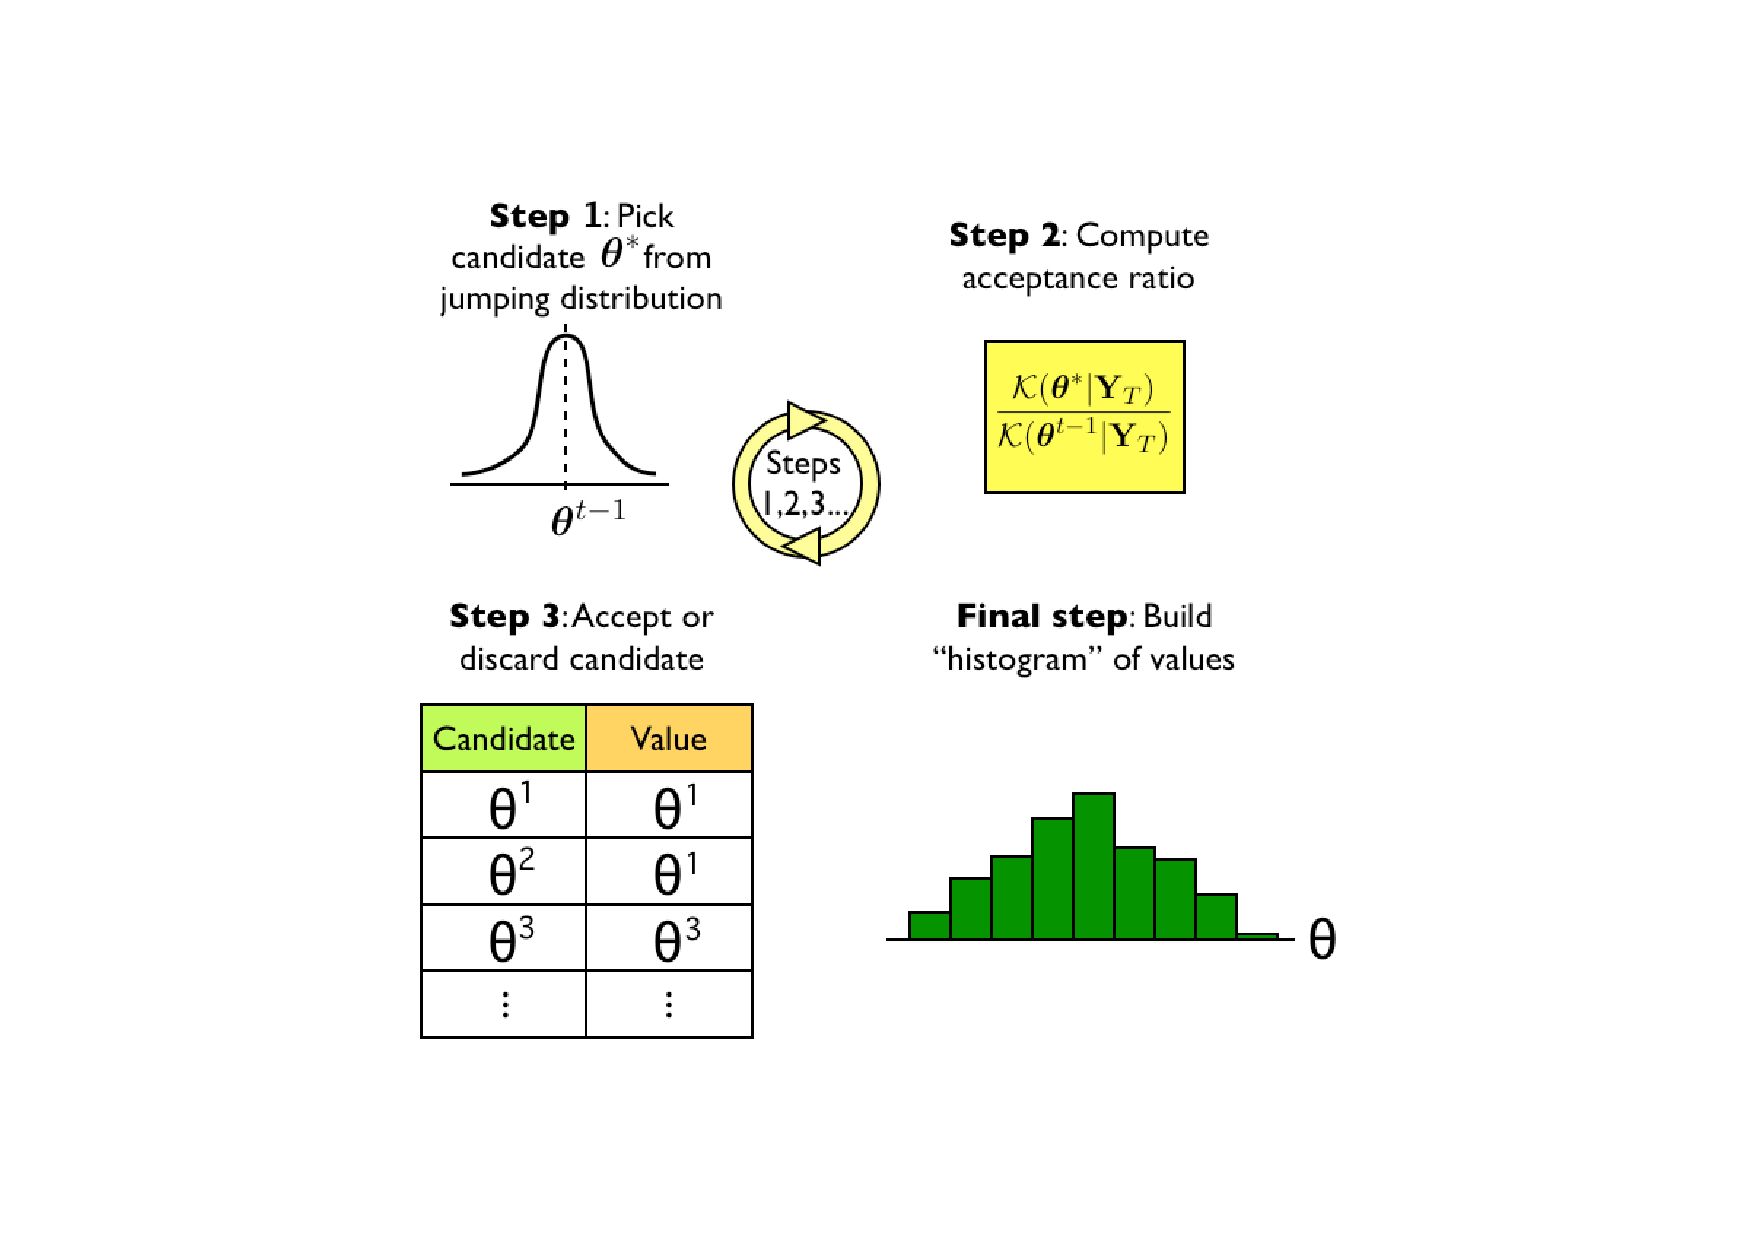
\includegraphics[width=1.0\textwidth]{P_MH2} 
\end{center} 
\caption[Illustration of the Metropolis-Hastings algorithm]{The above sketches the Metropolis-Hastings algorithm, used to build the posterior distribution function. Imagine repeating these steps a large number of times, and smoothing the ``histogram'' such that each ``bucket'' has infinitely small width.} 
\end{figure}

But why have such a complicated acceptance rule? The point is to be able to visit the entire domain of the posterior distribution. We should not be too quick to simply throw out the candidate giving a lower value of the posterior kernel, just in case using that candidate for the mean of the drawing distribution allows us to to leave a local maximum and travel towards the global maximum. Metaphorically, the idea is to allow the search to turn away from taking a small step up, and instead take a few small steps down in the hope of being able to take a big step up in the near future. Of course, an important parameter in this searching procedure is the variance of the jumping distribution and in particular the \textbf{scale factor}. If the scale factor is too small, the \textbf{acceptance rate} (the fraction of candidate parameters that are accepted in a window of time) will be too high and the Markov Chain of candidate parameters will ``mix slowly'', meaning that the distribution will take a long time to converge to the posterior distribution since the chain is likely to get ``stuck'' around a local maximum. On the other hand, if the scale factor is too large, the acceptance rate will be very low (as the candidates are likely to land in regions of low probability density) and the chain will spend too much time in the tails of the posterior distribution. \\

While these steps are mathematically clear, at least to a machine needing to undertake the above calculations, several practical questions arise when carrying out Bayesian estimation. These include: How should we choose the scale factor $c$ (variance of the jumping
        distribution)? What is a satisfactory acceptance rate? How many draws are ideal? How is convergence of the Metropolis-Hastings iterations assessed? These are all important questions that will come up in your usage of Dynare. They are addressed as clearly as possible in section \ref{sec:estimate} of Chapter \ref{ch:estbase}. \\

\section{Comparing models using posterior distributions}
As mentioned earlier, while touting the advantages of Bayesian estimation, the posterior distribution offers a particularly natural method of comparing models. Let's look at an illustration. \\

Suppose we have a prior distribution over two competing models: $p(\mathcal{A})$ and $p(\mathcal{B})$. Using Bayes' rule, we can compute the posterior
            distribution over models, where $\mathcal{I}=\mathcal{A},\mathcal{B}$ 
        \[
            p(\mathcal{I}|\mathbf Y_T) = \frac{p(\mathcal{I})p(\mathbf Y_T|\mathcal{I})}
            {\sum_{\mathcal{I}=\mathcal{A},\mathcal{B}}p(\mathcal{I})p(\mathbf Y_T|\mathcal{I})}
        \]
where this formula may easily be generalized to a collection of $N$ models.

Then, the comparison of the two models is done very naturally through the ratio of the posterior model distributions. We call this the \textbf{posterior odds ratio}:
        \[
            \frac{p(\mathcal{A}|\mathbf Y_T)}{p(\mathcal{B}|\mathbf
            Y_T)} = \frac{p(\mathcal{A})}{p(\mathcal{B})}
            \frac{p(\mathbf Y_T|\mathcal{A})}{p(\mathbf Y_T|\mathcal{B})}
        \]

The only complication is finding the magrinal density of the data conditional on the model, $p(\mathbf Y_T|\mathcal{I})$, which is also the denominator of the posterior density $p(\boldsymbol\theta | \mathbf Y_T)$ discussed earlier. This requires some detailed explanations of their own. \\

For each model $\mathcal{I}=\mathcal{A},\mathcal{B}$ we can evaluate, at least theoretically, the marginal
        density of the data conditional on the model by integrating out the deep parameters $\boldsymbol\theta_{\mathcal{I}}$ from the posterior kernel:
        \[
            p(\mathbf Y_T|\mathcal{I}) = \int_{\Theta_{\mathcal{I}}} p(\boldsymbol\theta_{\mathcal{I}}; \mathbf Y_T
            |\boldsymbol\theta_{\mathcal{I}},\mathcal{I}) d\boldsymbol\theta_{\mathcal{I}} = \int_{\Theta_{\mathcal{I}}} p(\boldsymbol\theta_{\mathcal{I}}|\mathcal{I})\times p(\mathbf Y_T
            |\boldsymbol\theta_{\mathcal{I}},\mathcal{I}) d\boldsymbol\theta_{\mathcal{I}}
        \]
Note that the expression inside the integral sign is exactly the posterior kernel. To remind you of this, you may want to glance back at the first subsection above, specifying the basic mechanics of Bayesian estimation.\\
        
        To obtain the marginal density of the data conditional on the model, there are two options. The first is to assume a functional form of the posterior kernel that we can integrate. The most straightforward and the best approximation, especially for large samples, is the Gaussian (called a \textbf{Laplace approximation}). In this case, we would have the following estimator:
\[
\widehat{p}(\mathbf Y_T|\mathcal I) = (2\pi)^{\frac{k}{2}}|\Sigma_{\boldsymbol\theta^m_{\mathcal I}}|^{\frac{1}{2}}p(\boldsymbol\theta_{\mathcal I}^m|\mathbf
Y_T,\mathcal I)p(\boldsymbol\theta_{\mathcal I}^m|\mathcal I)
\]
where $\boldsymbol\theta_{\mathcal I}^m$ is the posterior mode. The advantage of this technique is its computational efficiency: time consuming Metropolis-Hastings iterations are not necessary, only the numerically calculated posterior mode is required. \\

The second option is instead to use information from the Metropolis-Hastings runs and is typically referred to as the \textbf{Harmonic Mean Estimator}. The idea is to simulate the marginal density of interest and to simply take an average of these simulated values. To start, note that
\[
p(\mathbf{Y}_T|\mathcal I)=\mathbb{E}\left[\frac{f(\boldsymbol\theta_{\mathcal I})}{p(\boldsymbol\theta_{\mathcal I}|\mathcal I)
            p(\mathbf{Y}_T|\boldsymbol\theta_{\mathcal I},\mathcal I)}\biggl|\boldsymbol\theta_{\mathcal I},\mathcal I\biggr.\right]^{-1}
\]
where $f$ is a probability density function, since 
\[
                \mathbb{E}\left[\frac{f(\boldsymbol\theta_{\mathcal I})}{p(\boldsymbol\theta_{\mathcal I}|\mathcal I)
                p(\mathbf{Y}_T|\boldsymbol\theta_{\mathcal I},\mathcal I)}\biggl|\boldsymbol\theta_{\mathcal I},\mathcal I\biggr.\right]
                =
                \frac{\int_{\Theta_{\mathcal I}}f(\boldsymbol\theta)d\boldsymbol\theta}{\int_{\Theta_{\mathcal I}}p(\boldsymbol\theta_{\mathcal I}|I)
                p(\mathbf{Y}_T|\boldsymbol\theta_{\mathcal I},\mathcal I)d\boldsymbol\theta_{\mathcal I}}
\]
and the numerator integrates out to one (see\citet{Geweke1999} for more details). \\

This suggests the following estimator of the marginal
        density
        \[
            \widehat{p}(\mathbf{Y}_T|\mathcal I)= \left[\frac{1}{B}\sum_{b=1}^B
            \frac{f(\boldsymbol\theta_{\mathcal I}^{(b)})}{p(\boldsymbol\theta_{\mathcal I}^{(b)}|\mathcal I)
            p(\mathbf{Y}_T|\boldsymbol\theta_{\mathcal I}^{(b)},\mathcal I)}\right]^{-1}
        \]
where each drawn vector $\boldsymbol\theta_{\mathcal I}^{(b)}$ comes from the
        Metropolis-Hastings iterations and where the probability density function $f$ can be viewed as a weights on the posterior kernel in order to downplay the importance of extreme values of $\boldsymbol\theta$. \citet{Geweke1999} suggests to use a truncated Gaussian function, leading to what is typically referred to as the \textbf{Modified Harmonic Mean Estimator}. \\    
            
            
